\documentclass[conference]{IEEEtran}

\usepackage[T1]{fontenc}
\usepackage[utf8]{inputenc}
\usepackage{graphicx}
\usepackage{booktabs}
\usepackage{array}
\usepackage{url}
\usepackage[hidelinks]{hyperref}
\usepackage{cite}

\title{HarmonyXR GazePose-Context: A Unity-Based Proof-of-Concept for Multimodal Context Inference in XR Training}
\hypersetup{
  pdftitle={HarmonyXR GazePose-Context: A Unity-Based Proof-of-Concept for Multimodal Context Inference in XR Training},
  pdfauthor={Varun Siddaraju and Lavanya D.}
}

\author{
\IEEEauthorblockN{Varun Siddaraju}
\IEEEauthorblockA{varunsiddaraju@gmail.com}
\and
\IEEEauthorblockN{Lavanya D.}
\IEEEauthorblockA{lavanyad.insight@gmail.com}
}

\begin{document}
\maketitle

\begin{abstract}
Adaptive extended reality (XR) training systems require more than object interaction events; they must interpret whether a user is focused, distracted, transitioning between task steps, or inactive. This paper presents HarmonyXR GazePose-Context, a Unity and Meta Quest proof-of-concept that implements a phase-structured multimodal context pipeline for a guided XR sorting task. The implemented scope covers Phase 1 signal capture, Phase 2 feature extraction, Phase 2.3 context inference, and Phase 3 XR application adaptation. The system synchronizes gaze and AOI, head and body pose, hand, spatial, and task-progress evidence into runtime signal frames, derives modality-specific features, applies interpretable rule-based fusion, stabilizes context changes over time, and maps inferred states to in-headset guidance. On Meta Quest 2, gaze evidence is implemented as an application-level center-eye ray approximation rather than calibrated hardware eye tracking, which is not available on that device. The Unity 6 implementation was verified on Meta Quest 2 using ADB device evidence, Android package and activity dumps, Unity logcat output, and app-generated context JSONL logs. The May 20, 2026 evidence run produced 2,220 valid context records and observed all four target states: Engaged, Distracted, Transitioning, and Idle. This paper reports the implemented system's contribution and prototype validation evidence. Formal Phase 4 participant evaluation, baseline comparison, workload analysis, and statistical claims are treated as future work because completed user-study evidence is not yet available.
\end{abstract}

\begin{IEEEkeywords}
extended reality, adaptive XR, context inference, gaze, pose, hand tracking, multimodal interaction, Unity, Meta Quest
\end{IEEEkeywords}

\section{Introduction}
XR training environments are increasingly expected to respond to user attention, task flow, hesitation, and inactivity without requiring explicit status input. A conventional XR task can detect object collisions or button presses, but those events do not fully describe the user's state. For example, a user may look away from the task, pause before the next action, move between objects, or remain still without completing an interaction. These states matter for adaptive guidance because the appropriate support differs across focused work, distraction, transition, and inactivity.

HarmonyXR GazePose-Context addresses this problem through a Unity-based proof-of-concept for multimodal context inference. The prototype uses a deliberately simple sorting task in which the user places a cube, cylinder, and sphere into matching receptacles. The task is intentionally constrained so the research focus remains on context inference, signal fusion, and adaptive XR support rather than on game complexity.

The project follows a phase-structured implementation guide. Phase 1 captures gaze, head and body pose, hand, and spatial signals. Phase 2 converts raw signals into features. Phase 2.3 fuses features into context states. Phase 3 applies the inferred state inside the XR application layer. Phase 4, the formal participant study, is outside the completed scope reported in this paper.

The contributions are:
\begin{itemize}
\item a phase-structured Unity XR implementation for multimodal context inference;
\item a three-layer architecture separating sensor abstraction, context inference, and XR app adaptation;
\item an interpretable four-state context model for Engaged, Distracted, Transitioning, and Idle behavior;
\item an adaptive training shell that maps inferred context to in-headset guidance and support; and
\item a Quest evidence package showing activity launch, runtime logging, signal coverage, and all four target context states across 2,220 valid context records.
\end{itemize}

\section{Related Work}
\subsection{Gaze Tracking and Attention in VR}
Eye tracking and gaze-based interaction are central to attention-aware XR systems. Moreno-Arjonilla et al. survey VR eye-tracking hardware, calibration, gaze estimation, datasets, and applications, showing that gaze is a foundational signal for immersive attention analysis \cite{moreno2024eyetracking}. Pastel et al. compare gaze accuracy and precision in real and virtual environments and show that dynamic conditions can make gaze interpretation more difficult \cite{pastel2021gaze}. These findings support using gaze and AOI evidence in HarmonyXR while avoiding a gaze-only interpretation of context. Importantly, the current implementation targets Meta Quest 2, which does not provide hardware eye tracking; gaze evidence is therefore implemented as a center-eye ray approximation at the application level.

\subsection{Multimodal Attention and XR Interaction}
Multimodal sensing can reduce ambiguity that is present in any single signal. Long et al. show that EEG and eye-tracking features can improve classification of internal and external attention in VR \cite{long2024multimodal}. Rakkolainen et al. review multimodal interaction technologies across extended reality, including gaze, gesture, speech, haptics, and physiological sensing \cite{rakkolainen2021technologies}. Kim et al. describe the shift from controller-centered XR input toward hand, gaze, wrist, voice, and multimodal input across device generations \cite{kim2026controllers}. HarmonyXR follows this multimodal direction but emphasizes a lightweight behavioral pipeline that can run inside a Unity Quest prototype.

\subsection{Body, Head, and Hand Tracking}
Body and posture signals provide complementary evidence for user state. Bustamante et al. demonstrate skeleton-based posture recognition using lightweight geometric heuristics in a home care monitoring context, illustrating the broader utility of pose-based behavioral inference \cite{bustamante2025skeleton}. Neidhardt et al. show that XR body tracking can support movement analysis in VR-based musculoskeletal training \cite{neidhardt2023body}. Hand interaction is also important because pinch activity, object proximity, and interaction frequency indicate whether the user is actively engaging with task objects. Lei et al. present a sensor-fusion approach for precise hand tracking in VR \cite{lei2023hand}. HarmonyXR does not attempt to improve tracking accuracy itself; it uses available hand and pose evidence as part of a higher-level context model.

\subsection{Context-Aware Adaptation}
Gaze and context signals have been used to drive adaptive feedback and interface behavior. Selaskowski et al. present gaze-based attention refocusing training in VR for adults with ADHD \cite{selaskowski2023gaze}. Davari and Bowman propose a design space for context-aware XR interfaces and adaptive content placement \cite{davari2024context}. Ramiotis and Mania propose CONTEXT-GAD, a context-aware gaze adaptive dwell model for XR selection \cite{ramiotis2025contextgad}. These works show the value of context-aware XR, but many systems focus on interface placement or gaze selection. HarmonyXR instead implements a general task-context proof-of-concept that fuses gaze and AOI, pose, hand, spatial, and task evidence into four interpretable runtime states.

\section{Research Problem}
The research problem is: how can an XR training application infer task-relevant user context from lightweight runtime signals and use that inference to provide adaptive support without requiring explicit status input from the user?

The implemented proof-of-concept addresses this question at the systems level. It evaluates whether the planned architecture can be built, executed on a Quest headset, and validated through device-generated evidence. It does not claim that adaptive support improves learning, workload, or task performance because the planned Phase 4 user study has not yet been completed.

The implemented scope includes Unity and Meta Quest execution, the TrainingSimulation sorting task, four context states, runtime QA metrics, context-state logging, adaptive guidance, and device-side evidence collection. The excluded scope includes participant statistics, NASA-TLX analysis, formal ground-truth annotation, and baseline-versus-adaptive statistical comparison.

\section{System Overview}
The implementation follows the three-layer architecture defined by the project plan and implementation guide: Sensor Abstraction Layer, Context Engine Layer, and XR Application Layer. Fig.~\ref{fig:pipeline} summarizes the runtime pipeline.

\begin{figure}[t]
\centering
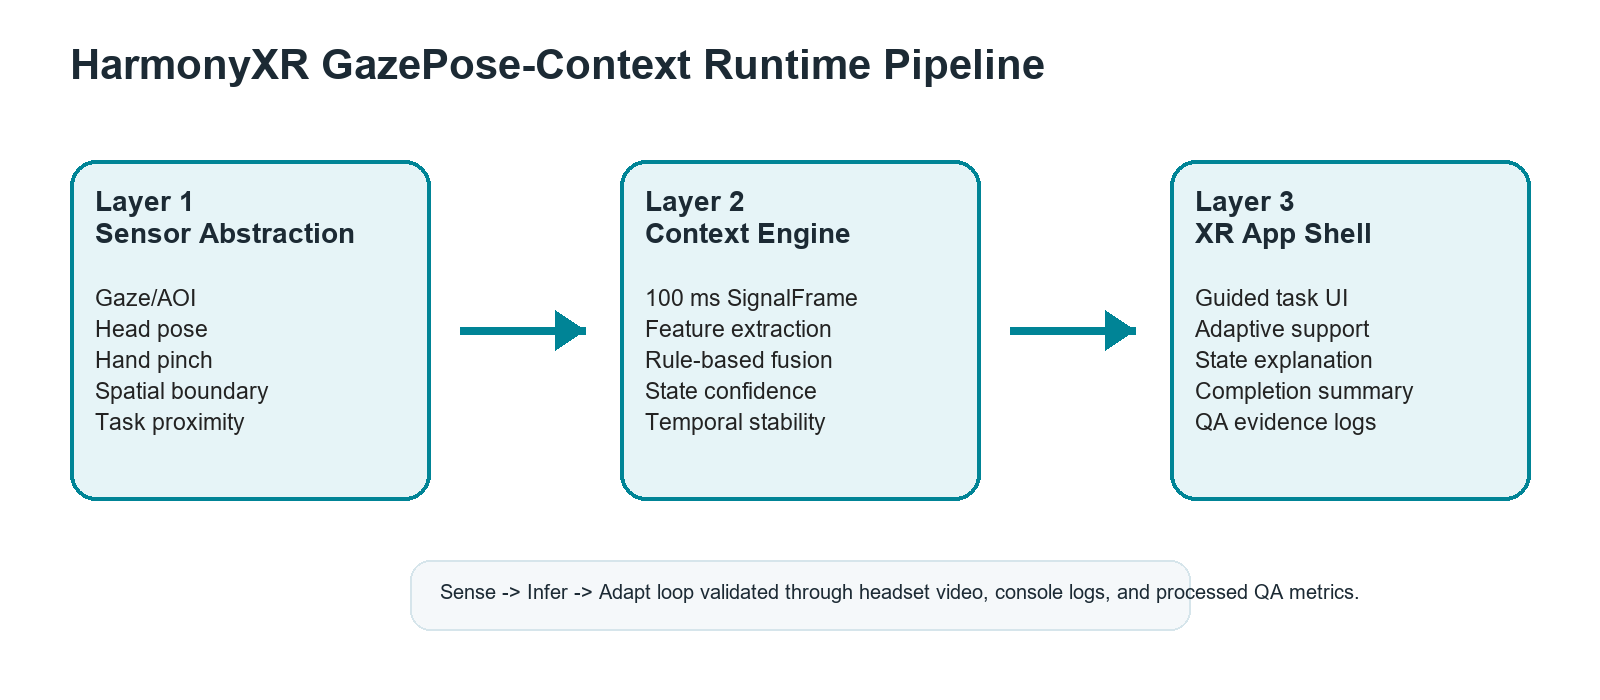
\includegraphics[width=\linewidth]{figures/figure1_runtime_pipeline.png}
\caption{HarmonyXR GazePose-Context runtime pipeline.}
\label{fig:pipeline}
\end{figure}

\subsection{Sensor Abstraction Layer}
The sensor abstraction layer corresponds to Phase 1 of the implementation plan. It captures gaze and AOI evidence, head and body pose evidence, hand activity, pinch state, object proximity, spatial context, and task-relevant scene information. On Meta Quest 2, which does not provide hardware eye tracking, gaze direction is approximated using the center-eye camera ray at the application level. The layer writes these values into a shared runtime signal frame so later stages do not depend directly on individual Unity components.

\subsection{Context Engine Layer}
The context engine combines Phase 2 feature extraction and Phase 2.3 context inference. Feature extractors convert raw signal values into gaze, body, hand, and spatial features. The context engine then applies interpretable fusion rules and a temporal state machine to infer a stable context state and confidence value.

\subsection{XR Application Layer}
The XR application layer corresponds to Phase 3. It consumes the inferred context state and updates the in-headset application behavior. This layer includes onboarding, task guidance, adaptive prompts, idle controls, completion messaging, QA output, and scene alignment behavior.

\section{Methodology}
The methodology follows the implementation guide's pipeline: signal acquisition, synchronization, feature extraction, multimodal fusion, temporal stabilization, adaptive response, and validation. The pipeline is rule-based rather than learned because the current project stage prioritizes inspectability, reproducibility, and traceable evidence mapping.

\subsection{Phase-Structured Implementation}
Phase 1 implements signal capture through gaze, body, hand, spatial, and synchronization scripts. Phase 2 implements feature extraction through gaze, body, hand, and body-hand feature extractors. Phase 2.3 implements context inference through the context engine, fusion engine, state machine, and context logger. Phase 3 implements the XR application shell through the app controller, adaptation manager, user guide, task manager, and supporting task-object scripts.

\subsection{Signal Acquisition and Synchronization}
The runtime collects signals from scene and headset components and synchronizes them into a common signal frame. The signal frame includes gaze origin and direction, AOI hit information, fixation-related timing, head pose, posture or spatial mode, hand pinch state, interaction count, nearest object distance, context state, confidence, previous state, hold duration, transition count, and nearest interactable.

The implementation guide expects synchronized processing rather than independent per-script interpretation. HarmonyXR follows this design by using \texttt{SignalSynchroniser} as the bridge from raw capture scripts to inference logic. This supports evidence review because context outputs can be traced back to the signal values available in the same runtime frame.

\subsection{Feature Extraction}
Gaze features include task AOI focus, fixation-on-AOI, fixation duration, dwell ratio, and saccade-like activity. Body and spatial features include posture or boundary context, locomotion activity, and movement values. Hand features include interaction frequency, pinch activity, and object proximity. These features convert low-level signals into inference-oriented evidence used by the context engine.

\subsection{Fusion and Stabilization}
The context engine applies prioritized rule-based fusion. Engaged is supported by task AOI focus, fixation or dwell evidence, active interaction, and low head-gaze divergence. Distracted is supported by lack of task AOI focus, low dwell, away evidence, and low interaction. Transitioning captures movement between task states, task-adjacent gaze, short fixation, changing proximity, or preparatory interaction. Idle captures low body movement, low hand activity, no object proximity, and little task-directed gaze.

The context state machine stabilizes outputs over time to reduce rapid UI flicker. A candidate state must persist for a minimum hold duration before replacing the active state, and the current state, confidence, previous state, and transition count are preserved for logging and adaptation.

\subsection{Validation Method}
Validation follows the implementation guide's QA gates rather than a completed participant protocol. The completed validation checks include Quest connection, APK installation, correct Unity activity launch, runtime context logging, state coverage, memory information, graphics information, thermal information, and error-log review. Evidence was collected through ADB commands and app-generated logs.

\section{Prototype Implementation}
The prototype is implemented in Unity 6000.4.7f1. The verified Quest build uses OpenXR 1.16.1, Meta XR Core SDK 201.0.0, XR Management 4.6.0, URP 17.4.0, Unity Input System 1.19.0, TextMeshPro 5.0.0, Unity UI 2.0.0, and OVRPlugin 1.201.0. The target device for the evidence run was Meta Quest 2.

The main runtime scene is TrainingSimulation. The user sorts three virtual objects, a cube, cylinder, and sphere, into corresponding receptacles. Task objects and receptacles are marked as areas of interest so gaze and AOI evidence can be related to the task.

During the Unity 6 migration, the Android entry activity was changed to UnityPlayerGameActivity. This was required because the previous AppUIGameActivity entry caused the APK to remain on the Quest loading screen. The migration also replaced the full Meta XR All-in-One dependency with Meta XR Core to avoid duplicate Oculus Android namespace conflicts while retaining the features needed by the current prototype.

The primary runtime components are:
\begin{itemize}
\item \textbf{SignalSynchroniser}: produces synchronized runtime signal frames.
\item \textbf{Gaze, body, hand, and spatial capture scripts}: collect Phase 1 runtime evidence.
\item \textbf{Feature extractors}: convert raw signals into task-relevant context features.
\item \textbf{ContextEngine and ContextFusionEngine}: infer context state and confidence.
\item \textbf{ContextStateMachine}: stabilizes state transitions.
\item \textbf{ContextLogger}: writes app-generated context JSONL evidence.
\item \textbf{XRAppShellController}: maintains the XR shell and runtime scene support.
\item \textbf{AdaptationManager}: maps context state to adaptive guidance behavior.
\item \textbf{TrainingSimulationUserGuide and TrainingSimulationTaskManager}: manage instructions, task progress, and completion flow.
\end{itemize}

\section{Context State Model}
The system infers four states:
\begin{itemize}
\item \textbf{Engaged}: the user appears focused on task-relevant objects, guidance, or active manipulation.
\item \textbf{Distracted}: attention appears shifted away from task-relevant content, with reduced task-directed evidence.
\item \textbf{Transitioning}: the user appears to be moving between objects, receptacles, task steps, or interaction targets.
\item \textbf{Idle}: low activity, little task-directed gaze, little interaction, or a pause state.
\end{itemize}

These categories are runtime interface states, not clinical or psychological labels. Their purpose is to select appropriate adaptive guidance. Engaged allows normal task flow, Distracted can trigger refocus support, Transitioning can support next-step movement, and Idle can trigger pause or continue controls.

\section{Evidence and Validation}
Evidence was collected from a Meta Quest 2 QA run on May 20, 2026 after the Unity 6 migration. The evidence package is retained in the project repository under a dedicated QA evidence directory. It includes ADB device output, device model and Android version, installed package details, Android activity dumps, runtime logcat, error-only logcat, memory information, graphics information, thermal status, app-generated context JSONL logs, a supporting legacy context JSON file, a state-count CSV, and a parsed context summary JSON.

ADB confirmed that the device was connected and that the Unity package was installed. Activity inspection confirmed launch through \texttt{UnityPlayerGameActivity}. Runtime logcat confirmed continuous Unity context output. The app-generated context JSONL file contained 2,220 valid records, and the parsed summary confirmed all four target context states.

\subsection{Validation Gates}
The completed validation gates were:
\begin{itemize}
\item Quest 2 detected through ADB;
\item package installed and discoverable on device;
\item Unity activity launch verified;
\item Unity runtime activity and context-log output were observed after launch;
\item TrainingSimulation generated runtime context records;
\item app-generated context JSONL log collected from device storage;
\item all four target context states found in parsed evidence;
\item memory, graphics, and thermal diagnostic files captured; and
\item error-only logcat reviewed for Unity package fatal errors.
\end{itemize}

\subsection{Evidence Boundary}
The evidence supports prototype runtime validity, not user-study effectiveness. It shows that the phase-defined system was implemented, executed on device, generated context records, and reached all target states. It does not establish classification accuracy against ground truth, workload reduction, learning benefit, or statistical improvement over a baseline.

\section{Results}
The May 20, 2026 Quest evidence run produced 2,220 valid JSONL context records. All four target states appeared in the app-generated evidence. Table~\ref{tab:statecoverage} reports the parsed state counts.

\begin{table}[t]
\centering
\caption{Context state coverage from headset runtime evidence.}
\label{tab:statecoverage}
\begin{tabular}{lrr}
\toprule
State & Samples & Found \\
\midrule
Engaged & 144 & Yes \\
Distracted & 620 & Yes \\
Transitioning & 530 & Yes \\
Idle & 926 & Yes \\
\midrule
Total & 2,220 & --- \\
\bottomrule
\end{tabular}
\end{table}

\begin{figure}[t]
\centering

\includegraphics[width=\linewidth]{figures/figure2_state_coverage.png}
\caption{Context state sample counts observed in the May 20 Quest evidence run.}
\label{fig:coverage}
\end{figure}

The observed distribution is consistent with a QA-style runtime session rather than a controlled participant trial. Idle was the most frequent state, followed by Distracted and Transitioning, while Engaged appeared less frequently. For the current proof-of-concept, the key result is full state reachability and device-side context-log generation, not an optimized behavioral frequency distribution.

\section{Discussion}
The implemented system demonstrates that a Unity XR prototype can be structured around a clear multimodal context pipeline and validated through headset-generated evidence. The phase separation is useful because it prevents the research logic from being buried inside UI code. Signal capture, feature extraction, context inference, and XR adaptation remain separate enough to inspect, debug, and extend.

The rule-based approach is appropriate for the current proof-of-concept because each state decision can be explained using available signal evidence. This is important for early-stage XR research where readers need to understand why the system produced a given state. At the same time, rule-based inference may not generalize as well as a learned model once larger labeled datasets become available.

The adaptive shell also addresses a practical research communication problem. A context engine without a visible application layer is difficult to evaluate without headset access. By mapping inferred state to visible guidance, idle controls, focus cues, and task messaging, the prototype makes the context model understandable inside the headset experience.

\section{Limitations}
This paper reports a proof-of-concept implementation and runtime evidence package, not a completed empirical user study. The results should not be interpreted as statistical evidence that adaptive XR improves task performance, workload, or learning outcomes.

Several implementation limitations remain. The task is deliberately simple, so ecological validity for richer training scenarios is limited. The context engine is manually authored and threshold-driven. The gaze and AOI path in this implementation uses an application-level center-eye ray approximation rather than a calibrated hardware eye-tracking path, because Meta Quest 2 does not provide hardware eye tracking. The \texttt{room\_scale} posture value represents spatial or boundary context rather than strict sitting or standing classification. The context log is JSONL-style runtime evidence rather than a single JSON array.

\section{Future Work}
The planned Phase 4 user study should be conducted only after participant evidence is available. That study should compare baseline and adaptive conditions, collect task completion time, sorting errors, context detection accuracy against ground truth, and subjective workload such as NASA-TLX. Only completed participant data should be used for statistical claims.

Future technical work should add explicit ground-truth annotation support, improve latency measurement, refine state-transition rules, expand visual-evidence documentation, and evaluate learned models against the current rule-based context engine. Longer-term extensions may include locomotion-aware refinement, face tracking, physiological signals, multi-user context modeling, and personalization of thresholds or adaptation policies.

\section{Conclusion}
HarmonyXR GazePose-Context implements a phase-structured Unity XR proof-of-concept for multimodal context inference and adaptive task guidance. The implemented system captures runtime signals, extracts features, fuses evidence into four interpretable context states, stabilizes transitions, logs context output, and maps state to adaptive XR behavior. The Unity 6 Quest evidence package confirms device execution, \texttt{UnityPlayerGameActivity} launch, app-generated context logging, and all four target states across 2,220 valid context records. The work provides a traceable systems prototype and evidence base for an IEEE-style XR research paper, while formal Phase 4 participant evaluation remains future work.

\section*{Acknowledgment}
The authors thank VeeRuby Technologies and the University of Victoria for supporting this research. The authors also thank the members of the HarmonyXR project team for their contributions to implementation, testing, and documentation throughout the project.

\begin{thebibliography}{11}

\bibitem{moreno2024eyetracking}
J. Moreno-Arjonilla, A. Lopez-Ruiz, J. R. Jimenez-Perez, J. E. Callejas-Aguilera, and J. M. Jurado, ``Eye-tracking on virtual reality: a survey,'' \emph{Virtual Reality}, vol. 28, article 38, 2024, doi: 10.1007/s10055-023-00903-y.

\bibitem{pastel2021gaze}
S. Pastel, C.-H. Chen, L. Martin, M. Naujoks, K. Petri, and K. Witte, ``Comparison of gaze accuracy and precision in real-world and virtual reality,'' \emph{Virtual Reality}, vol. 25, pp. 175--189, 2021, doi: 10.1007/s10055-020-00449-3.

\bibitem{long2024multimodal}
X. Long, S. Mayer, and F. Chiossi, ``Multimodal detection of external and internal attention in virtual reality using EEG and eye tracking features,'' in \emph{Proceedings of Mensch und Computer 2024 (MuC '24)}, 2024, doi: 10.1145/3670653.3670657.

\bibitem{rakkolainen2021technologies}
I. Rakkolainen, A. Farooq, J. Kangas, J. Hakulinen, J. Rantala, M. Turunen, and R. Raisamo, ``Technologies for multimodal interaction in extended reality: a scoping review,'' \emph{Multimodal Technologies and Interaction}, vol. 5, no. 12, article 81, 2021, doi: 10.3390/mti5120081.

\bibitem{kim2026controllers}
H. Kim, S. Lee, and C. Kang, ``From controllers to multimodal input: a chronological review of XR interaction across device generations,'' \emph{Sensors}, vol. 26, no. 1, article 196, 2026, doi: 10.3390/s26010196.

\bibitem{bustamante2025skeleton}
A. Bustamante, L. M. Belmonte, A. Pereira, R. Morales, and A. Fernandez-Caballero, ``Skeleton-based posture recognition for home care from virtual unmanned aerial vehicle,'' \emph{Expert Systems}, 2025, doi: 10.1111/exsy.70108.

\bibitem{neidhardt2023body}
M. Neidhardt, S. Gerlach, F. N. Schmidt, I. A. K. Fiedler, S. Grube, B. Busse, and A. Schlaefer, ``VR-based body tracking to stimulate musculoskeletal training,'' arXiv:2308.03375, 2023.
[Note: preprint; peer-reviewed publication status unconfirmed at time of submission.]

\bibitem{lei2023hand}
Y. Lei, Y. Deng, L. Dong, X. Li, X. Li, and Z. Su, ``A novel sensor fusion approach for precise hand tracking in virtual reality-based human-computer interaction,'' \emph{Biomimetics}, vol. 8, no. 3, article 326, 2023, doi: 10.3390/biomimetics8030326.

\bibitem{selaskowski2023gaze}
B. Selaskowski \emph{et al.}, ``Gaze-based attention refocusing training in virtual reality for adult attention-deficit/hyperactivity disorder,'' \emph{BMC Psychiatry}, vol. 23, article 74, 2023, doi: 10.1186/s12888-023-04551-z.

\bibitem{davari2024context}
S. Davari and D. A. Bowman, ``Towards context-aware adaptation in extended reality: a design space for XR interfaces and an adaptive placement strategy,'' arXiv:2411.02607, 2024, doi: 10.48550/arXiv.2411.02607.
[Note: preprint; peer-reviewed publication status unconfirmed at time of submission.]

\bibitem{ramiotis2025contextgad}
G. Ramiotis and K. Mania, ``CONTEXT-GAD: a context-aware gaze adaptive dwell model for gaze-based selections in XR environments,'' in \emph{Proceedings of the 31st ACM Symposium on Virtual Reality Software and Technology (VRST '25)}, 2025, doi: 10.1145/3756884.3766048.

\end{thebibliography}

\end{document}
